\documentclass[french]{beamer}
\usetheme{default}

\usepackage[T1]{fontenc}
\usepackage[utf8]{inputenc}
\usepackage{lmodern}
\usepackage{geometry}
\usepackage{babel}
\usepackage{graphicx}
\graphicspath{ {./images/} }

\usepackage{listings}

\usepackage{standalone}

\usepackage{tikz}
\usetikzlibrary{calc,trees,positioning,arrows,chains,shapes.geometric,%
	decorations.pathreplacing,decorations.pathmorphing,shapes,%
	matrix,shapes.symbols,fit,arrows.meta,backgrounds}


\title{Étude de quelques algorithmes de joueurs artificiels participants à des jeux de stratégie en temps réel}
\author{Dimitri \bsc{Cocheril-Crèvecœur}}
\begin{document}
\begin{frame}[plain]
    \maketitle
\end{frame}
\begin{frame}{Plan}
	
\end{frame}
\begin{frame}{StarCraft}
	\begin{figure}
		\centering
		\begin{minipage}{0.49\textwidth}
			\centering
			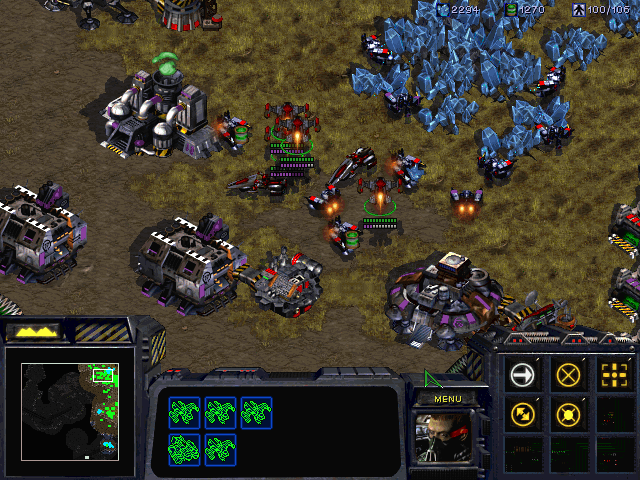
\includegraphics[width=0.95\textwidth]{screen_starcraft.png}
		\end{minipage}\hfill
		\begin{minipage}{0.49\textwidth}
			
		\end{minipage}
	\end{figure}
\end{frame}
\begin{frame}{Modèles existants}
	\begin{itemize}
		\item 
	\end{itemize}
\end{frame}
\begin{frame}{Développement moteur du jeu}
	\begin{figure}
		\centering
		\begin{minipage}{0.49\textwidth}
			\centering
			\includestandalone[width=\linewidth]{images/tikz_moteur}
		\end{minipage}\hfill
		\begin{minipage}{0.49\textwidth}
			\centering
			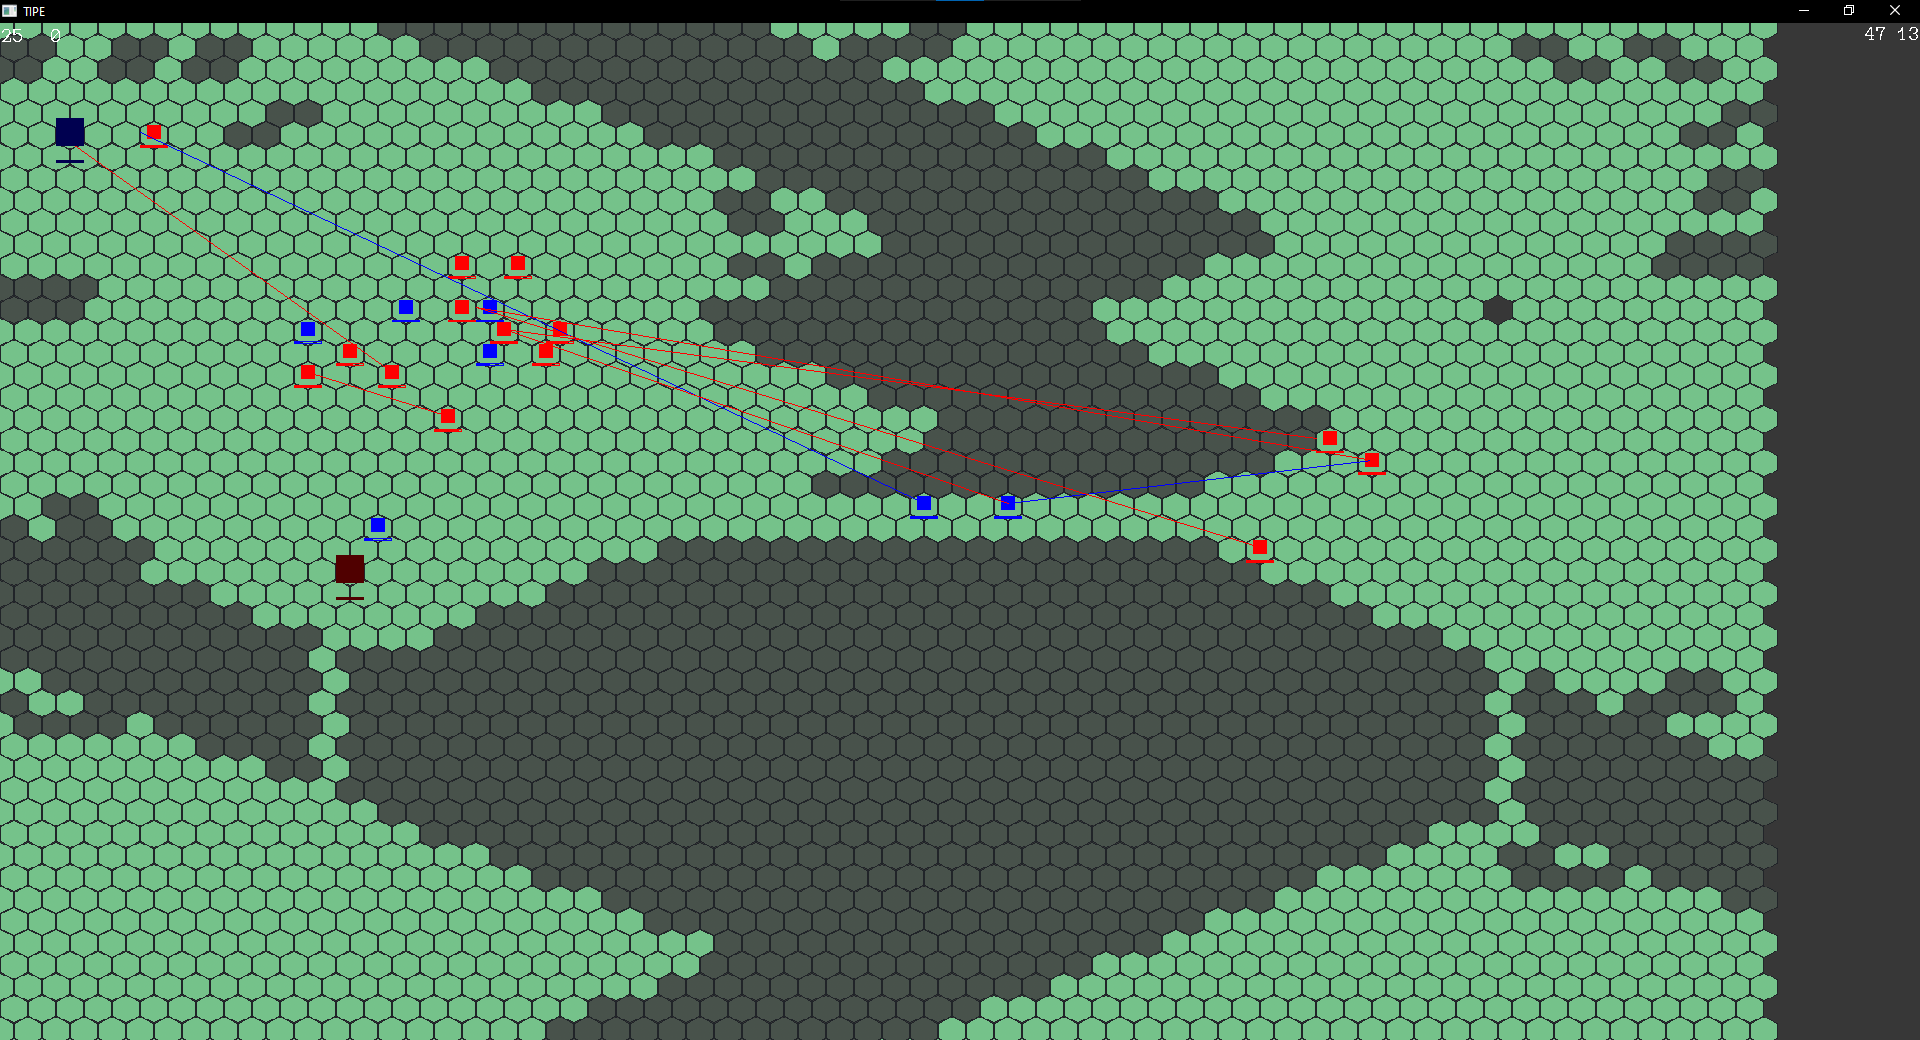
\includegraphics[width=0.95\textwidth]{screen_carte_pleine.png}
		\end{minipage}
	\end{figure}
\end{frame}
\begin{frame}[fragile]
	\small
	\begin{lstlisting}[language=C++,basicstyle=\ttfamily,keywordstyle=\color{red}]
void game_class::play() const
{
  for (const auto p : players_)
  // Pour chaque joueur...
  {
    p->moves_get(this, state_);
    // ..on choisit les actions..
  }
  state_->moves_make(map_);
  // ..et on effectue les actions.
}
	\end{lstlisting}
\end{frame}
\begin{frame}{Stratégie naïve : attaque par puissance}
	
\end{frame}
\begin{frame}{Stratégie naïve : attaquer par distance}
	
\end{frame}
\begin{frame}{Utilisation MCTS}
	
\end{frame}
\begin{frame}{Rassemblement des unitées : DBSCAN}
	
\end{frame}

\end{document}
